This section describes the relationships between the different classes
described in \cref{sub:pd_classes}. These relationships will be
visualised in a class diagram as described
in~\cite{mathiassen2001objektorienteret}.

The authors of~\cite{mathiassen2001objektorienteret} operate with three
main structuring techniques.

\begin{description}
\item[Generalisation] Generalisation is used to describe an \enquote{is a}
  relationship between classes. A class is called a
  superclass when another class inherits attributes and operations
  from this superclass. The other class is now a subclass of the
  superclass. In class diagrams, generalisation is denoted by a
  triangular arrow pointing from the subclass to the superclass.
\item[Aggregation] Aggregation is used to describe a
  \enquote{contains} relationship between classes. In class diagrams,
  aggregation is denoted by a rhombus shaped arrow.
\item[Association] Association is used to describe that two classes
  are aware of each other. Association is denoted in class diagrams by
  a line between each class.
\end{description}

Based on these structuring techniques, a class diagram, showing the
structure of the classes in the problem domain of the system, has been
made. See \cref{fig:pd_structure}. A \textit{User} can have an
association with a \textit{Vote}, i.e. they have voted on a track. A
\textit{Vote} then has an association with a \textit{Track} class. A
\textit{Track} can have many \textit{Vote} classes associated with
it.

A \textit{Playlist} contains one or more \textit{Track}s, i.e. the
tracks yet to be played. A \textit{Venue} has zero to many
restrictions on the music to be played there. A \textit{Venue} also
has exactly one \textit{Playlist}, containing the tracks that have
been voted for, and exactly one \textit{History} class that contains
the tracks that have been played in the past. Lastly, a \textit{Venue} is also associated zero to
many \textit{User}s, i.e the guests at the venue.

\begin{figure}[htbp]
  \centering
  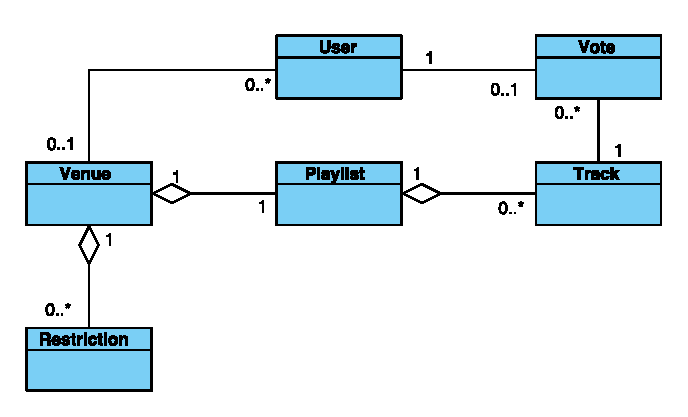
\includegraphics[width=\textwidth]{ProblemAreaClassDiagram.pdf}
  \caption{Class diagram of the problem domain.}\label{fig:pd_structure}
\end{figure}
